\chapter{Hauptteil/Main Part}

\section{Hardware}
\subsection{Breadboard Prototype}
Our prototype uses the NodeMCU ESP32 development board by Joy-IT. The board is equipped with the ESP32-WROOM-32 module. ESP32-WROOM-32 is a powerful, generic Wi-Fi+BT+BLE MCU module. 

At the core of the module is the ESP32-D0WDQ6 chip \cite[6]{esp32-module}. This chip, and therefore this module. is not recommended for new designs anymore due to chip revisions. The ESP32-D0WDQ6 is based on chip revision v.1.0 or v1.1. \cite[11]{esp32-datasheet}. The ESP32-WROOM-32 module could therefore be replaced by the newer ESP32-WROOM-32E module. The ESP32-WROOM-32E module uses a ESP32-D0WD-V3 or ESP32-D0WDR2-V3 chip which are based on chip revision v3.0 or v3.1 which fixes some Hardware bugs \cite[1]{esp32-module-new}, \cite[11]{esp32-datasheet}, \cite[3-4]{esp32-errata}. Compared to the ESP32-WROOM-32 module, the ESP32-WROOM-32E module has versions that provide additional 2MB PSRAM, support higher operating ambient temperatures and veWrsions with higher integrated SPI flash sizes (8MB or 16MB) \cite[2]{esp32-module-new}, \cite[6-7]{esp32-module}.

\subsection{Cryptographic Hardware accelerators}
\begin{figure}
	\centering
	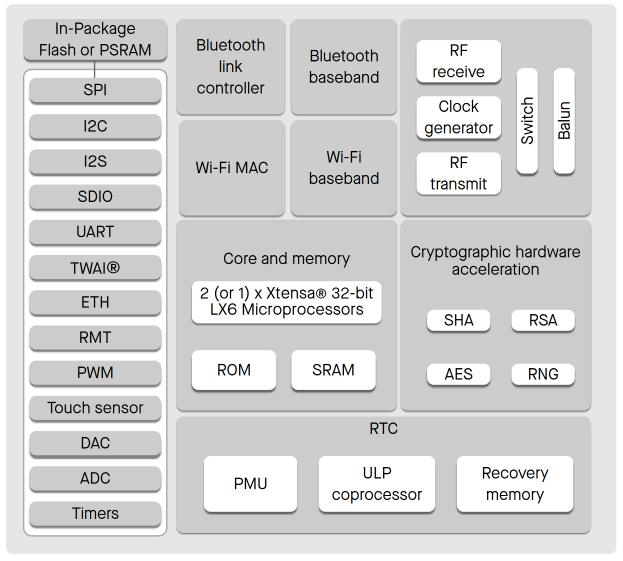
\includegraphics[scale=.5]{abbildungen/functional-block-diagram}
	\caption{ESP32 Functional Block Diagram}
	\label{Fig:esp32-crypto}
\end{figure}



\section{Implementation/Software Architecture}
\subsection{Model}
\subsubsection{Difference with other Implementations}
Since ElectionGuards original specification in 2019, there have been several implementations of ElectionGuard that have been used in various applications \cite[eg-paper]. The current roadmap of ElectionGuard targets a c++ implementation of the ElectionGuard 2.0 specification. [https://www.electionguard.vote/overview/Roadmap/]. Earlier implementations include a Python reference implementation of the ElectionGuard 1.0 specification and an encryption engine in C++ with a C wrapper.

ESP32 development support development of applications in C, C++ and Micropython. [source]. Initialy, we could try to port the encryption engine written in c++ over to ESP32. This would allow us to use the existing codebase and focus on the integration of the encryption component with the hardware.
The encryption engine would be responsible for generating an elgamal keypair and the subsequent exchange of cryptographic proofs and cryptographic keys. 

The modular exponentiation at the heart of most ElectionGuard operations imposes the highest computaitional cost among all computations and is the limiting factor in any performance analysis. Using fast libraries for modular arithmetic is crucial to achieve good performance so that the latency due to Key generation and ZK proof generation doesn not impact usability. [source]

The c++ implementation uses Microsoft's HACL* - a performant C implementation of a wide variety of cryptographic primitives which have been formally verified for correctness [source.]. For performance reasons the implementation of the c++ encryption engine  uses pre-computed tables to make encryption substantially faster. This is possible because most exponentiations in ElectionGuard have fixed base, either the generator g or the election public key K. The pre-computed tables contain certain powers of these bases. The Python reference implementation uses a more straightforwar approach by using GnuMP. [source].

The ESP32 is equipped with hardware accelerators of general algorithms such as SHA and RSA and it also supports independent arithmetic, such as Big Integer Multiplication and Big Integer Modular Multiplication. [esp tech reference,4.1.19]. The hardware accelerators greatly improve operation speed and reduce software complexity. 

\subsubsection{Performance}
- With/Without HW Accerleration
- Single/Dual Core
\subsection{View}
\subsection{Adapter}

\section{Verification}









\begin{table}[ht]
	\centering
	\begin{tabular}{|c|c|c|c|}
		\hline
		&LCD&Board&Description\\\hline
		1&VCC&3.3V\\\hline
		2&GND&GND\\\hline
		3&GND&GND\\\hline
		4&NC \\\hline
		5&NC \\\hline
		6&NC \\\hline
		7&CLK&D14&SPI-CLK\\\hline
		8&SDA&D13&SPI-MOSI\\\hline
		9&RS&D34&Any GPIO PIN\\\hline
		10&RST&D35&Any GPIO PIN\\\hline
		11&CS&D15&SPI-SS\\\hline
	\end{tabular}
	\caption{PINOUT LCD}
	\label{Tab:PINOUT_LCD}
\end{table}

Bachelor- und Masterarbeiten können sowohl in deutsch als auch in englisch geschrieben werden. 
Die sprachliche Ausarbeitung wird bewertet, was bei der Wahl der Sprache berücksichtigt werden sollte. 
Im folgenden werden ein paar Hinweise zur Ausarbeitung  mit \LaTeX\ gegeben.


\section{Unterkapitel}
\subsection{Dritte Gliederungsebene}
Falls in einem Kapitel mehrere Gliederungsebenen verwendet werden sollte darauf geachtet werden, dass mindestens drei Punkte pro ebene existieren. 

\begin{table}[h]
	\centering
	\begin{tabular}{|l|l|l|}
		\hline
		1&2&3\\\hline
		4&5&6\\\hline
	\end{tabular}
	\caption{Beispieltabelle}
	\label{Tab:Beispieltabelle}
\end{table}

Hier wird die Beispieltabelle~\ref{Tab:Beispieltabelle} referenziert.

\begin{figure}[h] %in den eckigen Klammern wird angegeben, wo das Bild erscheinen soll:
	%h = here, t = top, b = bottom, p = page (eigene Seite für Bild/er)
	%TeX versucht es in dieser Reihenfolge schön hinzukriegen
	%wenn das erste gut aussieht, wird das genommen, sonst das zweite usw.
	\centering
	
\includegraphics[scale=.25]{abbildungen/bild1}
	\caption[Bildunterschrift mit Quellenangabe]{Bildunterschrift mit Quellenangabe \cite{lcd}}
	\label{Fig:Bildbezeichnung}
\end{figure}

Hier wird die Beispielbild~\ref{Fig:Bildbezeichnung} referenziert.

\begin{equation} \label{eq:Beispielformel}
	\sum_{x=0}^{10}x=55
\end{equation}

Hier wird die Beispielformel~\ref{eq:Beispielformel} referenziert.

\textit{kursiv}, \textbf{fett}, \underline{unterstrichen}

Abkürzungen müssen im Abkürzungsverzeichnis angelegt werden.
Erste Verwendung einer \ac{ABK} jede weitere Verwendung der \ac{ABK}.

%Befehl um sämtliche Literatur im Literaturverzeichnis aufzuführen
\nocite{*}

